\documentclass[
  a4paper,
  oneside,
  BCOR = 10mm,
  DIV = 12,
  12pt,
  headings = normal,
]{scrartcl}

%%% Length calculations
\usepackage{calc}
%%%

%%% Support for color
\usepackage{xcolor}
\definecolor{lightblue}{HTML}{03A9F4}
\definecolor{red}{HTML}{F44336}
%%%

%%% Including graphics
\usepackage{graphicx}
%%%

%%% Font selection
\usepackage{fontspec}

\setromanfont{STIX Two Text}[
  SmallCapsFeatures = {LetterSpace = 8},
]

\setsansfont{IBM Plex Sans}[
  Scale = MatchUppercase,
]

\setmonofont{IBM Plex Mono}[
  Scale = MatchUppercase,
]
%%%

%%% Math typesetting
\usepackage{amsmath}
\usepackage{mathtools}

\usepackage{unicode-math}
\setmathfont{STIX Two Math}

\usepackage{IEEEtrantools}
%%%

%%% List settings
\usepackage{enumitem}
\setlist[enumerate]{
  label*      = {\arabic*.},
  left        = \parindent,
  topsep      = 0\baselineskip,
  parsep      = 0\baselineskip,
  noitemsep, % override itemsep
}
% List settings for levels 2–4
\setlist[enumerate, 2, 3, 4]{
  label*      = {\arabic*.},
  left        = 0em,
  topsep      = 0\baselineskip,
  parsep      = 0\baselineskip,
  noitemsep, % override itemsep
}

\setlist[itemize]{
  label*      = {—},
  left        = \parindent,
  topsep      = 0\baselineskip,
  parsep      = 0\baselineskip,
  itemsep     = 1\baselineskip,
  noitemsep, % override itemsep
}

\setlist[description]{
  font        = {\rmfamily\upshape\bfseries},
  topsep      = 1\baselineskip,
  parsep      = 0\baselineskip,
  itemsep     = 0\baselineskip,
}

%%%

%%% Structural elements typesetting
\setkomafont{pagenumber}{\rmfamily\upshape}
\setkomafont{disposition}{\rmfamily\bfseries}

% Sectioning
\RedeclareSectionCommand[
  beforeskip = -1\baselineskip,
  afterskip  = 1\baselineskip,
  font       = {\normalsize\bfseries\scshape},
]{section}

\RedeclareSectionCommand[
  beforeskip = -1\baselineskip,
  afterskip  = 1\baselineskip,
  font       = {\normalsize\bfseries\itshape},
]{subsection}

\RedeclareSectionCommand[
  beforeskip = -1\baselineskip,
  afterskip  = 1\baselineskip,
  font       = {\normalsize\bfseries},
]{subsubsection}

\RedeclareSectionCommand[
  beforeskip = -1\baselineskip,
  afterskip  = -0.5em,
  font       = {\normalsize\mdseries\scshape\addfontfeatures{Letters = {UppercaseSmallCaps}}},
]{paragraph}
%%%

%%% Typographic enhancements
\usepackage{microtype}
%%%

%%% Language-specific settings
\usepackage{polyglossia}
\setmainlanguage{ukrainian}
\setotherlanguages{english}
%%%

%%% Captions
\usepackage{caption}
\usepackage{subcaption}

%\DeclareCaptionLabelFormat{closing}{#2)}
%\captionsetup[subtable]{labelformat = closing}

%\captionsetup[subfigure]{labelformat = closing}

\captionsetup[table]{
  aboveskip = 0\baselineskip,
  belowskip = 0\baselineskip,
}

\captionsetup[figure]{
  aboveskip = 1\baselineskip,
  belowskip = 0\baselineskip,
}

\captionsetup[subfigure]{
  labelformat = simple,
  labelformat = brace,
  justification = RaggedRight,
  singlelinecheck = false,
}
%%%

%%% Hyphenated ragged typesetting
\usepackage{ragged2e}
%%%

%%% Table typesetting
\usepackage{booktabs}
\usepackage{longtable}

\usepackage{multirow}

\usepackage{array}
\newcolumntype{v}[1]{>{\RaggedRight\arraybackslash\hspace{0pt}}p{#1}}
\newcolumntype{b}[1]{>{\Centering\arraybackslash\hspace{0pt}}p{#1}}
\newcolumntype{n}[1]{>{\RaggedLeft\arraybackslash\hspace{0pt}}p{#1}}
%%%

%%% Drawing
\usepackage{tikz}
\usepackage{tikzscale}
\usetikzlibrary{datavisualization}
\usetikzlibrary{datavisualization.formats.functions}
\usetikzlibrary{positioning}
\usetikzlibrary{patterns}
\usetikzlibrary{intersections}
\usetikzlibrary{arrows.meta} % Stealth arrow tips
\usetikzlibrary{graphs}
\usetikzlibrary{graphdrawing}
\usegdlibrary{layered}
\usetikzlibrary{quotes}

\usepackage{pgfplots}
\usepgfplotslibrary{fillbetween}
%%%

%%% SI units typesetting
\usepackage{siunitx}
\sisetup{
  output-decimal-marker = {,},
  exponent-product      = {\cdot},
  inter-unit-product    = \ensuremath{{} \cdot {}},
  per-mode              = symbol,
}
%%%

% Code Highlighting
\usepackage{minted}
\setmintedinline{
  style = bw,
  breaklines,
}

\newminted[bashterm]{text}{%
  autogobble,%
  breaklines,%
  style=bw,%
}

\newminted[codegeneric]{text}{%
  autogobble,%
  style=bw,%
  breaklines,%
  fontsize=\small,%
}

\newmintinline{bash}{%
}

\newmintinline[minttext]{text}{%
  breaklines,%
  breakanywhere,%
}

%%% Framing code listings
\usepackage{tcolorbox}
\tcbuselibrary{breakable}
\tcbuselibrary{minted}
\tcbuselibrary{skins}

% Text file listing
\newtcblisting[
  auto counter,
  list inside,
  number within = section,
]{listingplaintext}[3][]{%
  minted language = text,
  minted style    = bw,
  minted options  = {
    autogobble,
    linenos,
    tabsize = 4,
    breaklines,
    breakanywhere,
    fontsize = \footnotesize,
  },
  empty,
  sharp corners,
  coltitle = black,
  borderline horizontal = {1pt}{0pt}{black},
  titlerule = {0.5pt},
  titlerule style = {
    black,
  },
  toptitle = 0.3em,
  bottomtitle = 0.3em,
  before skip      = \intextsep,
  after  skip      = \intextsep,
  title            = {Лістинг \thetcbcounter: #2},
  list entry       = {\protect\numberline{\thetcbcounter}#2},
  left = 0em,
  right = 0em,
  %
  listing only,
  breakable,
  %
  label = {#3},%
}

\newtcbinputlisting[
  use counter from = listingplaintext,
  list inside,
  number within = section
]{\inputplaintext}[4][]{%
  minted language = text,
  minted style    = bw,
  minted options  = {
    autogobble,
    linenos,
    tabsize = 4,
    breaklines,
    breakanywhere,
    fontsize = \footnotesize,
  },
  empty,
  sharp corners,
  coltitle = black,
  borderline horizontal = {1pt}{0pt}{black},
  titlerule = {0.5pt},
  titlerule style = {
    black,
  },
  toptitle = 0.3em,
  bottomtitle = 0.3em,
  before skip      = \intextsep,
  after  skip      = \intextsep,
  title            = {Лістинг \thetcbcounter: #3},
  list entry       = {\protect\numberline{\thetcbcounter}#3},
  left = 0em,
  right = 0em,
  %
  listing file={#2},
  listing only,
  breakable,
  %
  label = {#4}
}

\newtcblisting[
  use counter from = listingplaintext,
  list inside,
  number within = section,
]{listingpython}[3][]{%
  minted language = python,
  minted style    = bw,
  minted options  = {
    autogobble,
    linenos,
    tabsize = 4,
    breaklines,
    breakanywhere,
    fontsize = \footnotesize,
  },
  empty,
  sharp corners,
  coltitle = black,
  borderline horizontal = {1pt}{0pt}{black},
  titlerule = {0.5pt},
  titlerule style = {
    black,
  },
  toptitle = 0.3em,
  bottomtitle = 0.3em,
  before skip      = \intextsep,
  after  skip      = \intextsep,
  title            = {Лістинг \thetcbcounter: #2},
  list entry       = {\protect\numberline{\thetcbcounter}#2},
  left = 0em,
  right = 0em,
  %
  listing only,
  breakable,
  %
  label = {#3},
  %
  #1%
}

\newtcbinputlisting[
  use counter from = listingplaintext,
  list inside,
  number within = section
]{\inputpython}[4][]{%
  minted language = python,
  minted style    = bw,
  minted options  = {
    autogobble,
    linenos,
    tabsize = 4,
    breaklines,
    breakanywhere,
    fontsize = \footnotesize,
  },
  empty,
  sharp corners,
  coltitle = black,
  borderline horizontal = {1pt}{0pt}{black},
  titlerule = {0.5pt},
  titlerule style = {
    black,
  },
  toptitle = 0.3em,
  bottomtitle = 0.3em,
  before skip      = \intextsep,
  after  skip      = \intextsep,
  title            = {Лістинг \thetcbcounter: #3},
  list entry       = {\protect\numberline{\thetcbcounter}#3},
  left = 0em,
  right = 0em,
  %
  listing file={#2},
  listing only,
  breakable,
  %
  label = {#4}
}

% Linux command-line listing
\newtcblisting{linuxterm}%
{%
  % Syntax highlighing options
  listing only,%
  minted language = bash,%
  minted options={%
    autogobble,%
    linenos%
  },%
  % Presentation options
  empty,%
  %% Margins
  sharp corners,%
  toptitle = 0.0em,%
  bottomtitle = 0.0em,%
  left = 0em,%
  right = 0em,%
  before skip = \intextsep,%
  after skip = \intextsep,%
}

\newtcblisting{linuxtermout}%
{%
  % Syntax highlighing options
  listing only,%
  minted language = text,%
  minted options={%
    autogobble,%
    linenos%
  },%
  % Presentation options
  empty,%
  %% Margins
  sharp corners,%
  toptitle = 0.0em,%
  bottomtitle = 0.0em,%
  left = 0em,%
  right = 0em,%
  before skip = \intextsep,%
  after skip = \intextsep,%
}

% Dockerfile listings
\newtcblisting[
  use counter from = listingplaintext,
  list inside,
  number within = section,
]{listingdocker}[3][]{%
  minted language = dockerfile,
  minted style    = bw,
  minted options  = {
    autogobble,%
    linenos,
    tabsize = 4,
    breaklines,
    breakanywhere,
    fontsize = \footnotesize,
  },
  empty,
  sharp corners,
  coltitle = black,
  borderline horizontal = {1pt}{0pt}{black},
  titlerule = {0.5pt},
  titlerule style = {
    black,
  },
  toptitle = 0.3em,
  bottomtitle = 0.3em,
  before skip      = \intextsep,
  after  skip      = \intextsep,
  title            = {Лістинг \thetcbcounter: #2},
  list entry       = {\protect\numberline{\thetcbcounter}#2},
  left = 0em,
  right = 0em,
  %
  listing only,
  breakable,
  %
  label = {#3},%
}

% Docker Compose listings
\newtcblisting[
  use counter from = listingplaintext,
  list inside,
  number within = section,
]{listingdockercompose}[3][]{%
  minted language = yaml,
  minted style    = bw,
  minted options  = {
    autogobble,%
    linenos,
    tabsize = 4,
    breaklines,
    breakanywhere,
    fontsize = \footnotesize,
  },
  empty,
  sharp corners,
  coltitle = black,
  borderline horizontal = {1pt}{0pt}{black},
  titlerule = {0.5pt},
  titlerule style = {
    black,
  },
  toptitle = 0.3em,
  bottomtitle = 0.3em,
  before skip      = \intextsep,
  after  skip      = \intextsep,
  title            = {Лістинг \thetcbcounter: #2},
  list entry       = {\protect\numberline{\thetcbcounter}#2},
  left = 0em,
  right = 0em,
  %
  listing only,
  breakable,
  %
  label = {#3},%
}

% SWI Prolog listings
\newtcblisting[
  use counter from = listingplaintext,
  list inside,
  number within = section,
]{listingprolog}[3][]{%
  minted language = prolog,
  minted style    = bw,
  minted options  = {
    autogobble,%
    linenos,
    tabsize = 4,
    breaklines,
    breakanywhere,
    fontsize = \footnotesize,
  },
  empty,
  sharp corners,
  coltitle = black,
  borderline horizontal = {1pt}{0pt}{black},
  titlerule = {0.5pt},
  titlerule style = {
    black,
  },
  toptitle = 0.3em,
  bottomtitle = 0.3em,
  before skip      = \intextsep,
  after  skip      = \intextsep,
  title            = {Лістинг \thetcbcounter: #2},
  list entry       = {\protect\numberline{\thetcbcounter}#2},
  left = 0em,
  right = 0em,
  %
  listing only,
  breakable,
  %
  label = {#3},%
}

\newtcbinputlisting[
  use counter from = listingplaintext,
  list inside,
  number within = section
]{\inputprolog}[4][]{%
  minted language = prolog,
  minted style    = bw,
  minted options  = {
    autogobble,
    linenos,
    tabsize = 4,
    breaklines,
    breakanywhere,
    fontsize = \footnotesize,
  },
  empty,
  sharp corners,
  coltitle = black,
  borderline horizontal = {1pt}{0pt}{black},
  titlerule = {0.5pt},
  titlerule style = {
    black,
  },
  toptitle = 0.3em,
  bottomtitle = 0.3em,
  before skip      = \intextsep,
  after  skip      = \intextsep,
  title            = {Лістинг \thetcbcounter: #3},
  list entry       = {\protect\numberline{\thetcbcounter}#3},
  left = 0em,
  right = 0em,
  %
  listing file={#2},
  listing only,
  breakable,
  %
  label = {#4}
}


% Customize minted line numbers
\renewcommand{\theFancyVerbLine}{\ttfamily\scriptsize\arabic{FancyVerbLine}}

%%%

%%% Typeset menus and keys
\usepackage{menukeys}[
  os=win,
]
%%%

%%% Links and hyperreferences
\usepackage{hyperref}
\hypersetup{
  bookmarksnumbered = true,
  colorlinks      = false,
  linkbordercolor = red,
  urlbordercolor  = lightblue,
  pdfborderstyle  = {/S/U/W 1.5},
}
%%%

%%% Length adjustment

% Set baselineskip, default is 14.5 pt
\linespread{1.068966} % ~15.5 pt
\setlength{\emergencystretch}{1em}
\setlength{\parindent}{1.5em}
\newlength{\gridunitwidth}
\setlength{\gridunitwidth}{\textwidth / 12}
%%%

%%% Custom commands
\newcommand{\allcaps}[1]{%
  {%
    \addfontfeatures{%
      Letters = UppercaseSmallCaps,
      LetterSpace = 8,%
    }%
    #1%
  }%
}
\newcommand{\filename}[1]{\texttt{#1}}
\newcommand{\progname}[1]{\texttt{#1}}
\newcommand{\commandname}[1]{\texttt{#1}}
\newcommand{\modulename}[1]{\texttt{#1}}
\newcommand{\transeng}[1]{{англ.}~\textit{\textenglish{#1}}}
%%%

%%% Custom math commands
\newcommand{\longvar}[1]{\mathit{#1}}
\newcommand{\vect}[1]{\mathbfit{#1}}
\newcommand{\matr}[1]{\mathbfit{#1}}

\newcommand{\logequiv}{\mathrel{\Longleftrightarrow}} % Logically equivalent

\newcommand{\ssep}{\mid} % set builder separator

\DeclareMathOperator*{\minimize}{min} % minimize for linear programs
\DeclareMathOperator*{\rand}{rand} % rand()

\DeclarePairedDelimiter{\setpower}{\lvert}{\rvert} % set power
%%%

\begin{document}

\begin{titlepage}
    \begin{center}
      Міністерство освіти і~науки України\\
      Національний авіаційний університет\\
      Факультет кібербезпеки, комп'ютерної та~програмної інженерії\\
      Кафедра комп'ютеризованих систем управління

      \vspace{\fill}
        Лабораторна робота №~8\\
        з~дисципліни «Системи штучного інтелекту»\\
        на~тему «Штучні нейронні мережі. Моделювання логічних функцій»\\
        Варіант №~8

      \vspace{\fill}

      \begin{flushright}
        Виконав:\\
        студент \allcaps{ФККПІ}\\
        групи \allcaps{СП}-425\\
        Клокун В.\,Д.\\
        Перевірила:\\
        Яковенко Л.\,В.
      \end{flushright}

      Київ 2020
    \end{center}
  \end{titlepage}

  \section{Мета роботи}
    Отримати початкові навички по~створенню штучних нейронних мереж, що~здатні виконувати прості логічні функції.

  \section{Хід~роботи}
    За~завданням варіанту необхідно написати програму, яка~моделюватиме логічні функції \allcaps{І}, \allcaps{АБО}, \allcaps{НЕ} та~виключне~\allcaps{АБО}. Крім того, щоб~отримати максимальний бал, необхідно також змоделювати логічну функцію, яка~має~задану таблицю істинності~(табл.~\ref{tab:truth-table}).

    \begin{table}[!htbp]
      \caption{Таблиці істинності цільової логічної функції}
      \label{tab:truth-table}
      \begin{tabular}{
        *{3}{v{3\gridunitwidth - 2\tabcolsep}}
        *{1}{n{3\gridunitwidth - 2\tabcolsep}}
      }
        \toprule
          $x_1$ & $x_2$ & $x_3$ & $Y(x_1, x_2, x_3)$ \\
        \midrule
          0 & 0 & 0 & 1 \\
          0 & 1 & 0 & 1 \\
          1 & 0 & 0 & 0 \\
          1 & 1 & 1 & 1 \\
        \bottomrule
      \end{tabular}
    \end{table}

    Щоб~змоделювати звичайні логічні функції, досить використати параметри нейронів із~завдання на~лабораторну роботу. Однак для~заданої функції необхідно визначити параметри нейронної мережі самостійно.

    Так~як~функція задана неповною таблицею, її~значення для~інших наборів вхідних даних нас~не~цікавлять і~можуть бути довільними. Тому спробуємо змоделювати її~за~допомогою одного нейрона з~3~входами. Щоб~змоделювати логічну функцію, необхідно визначити ваги входів~$w_i$ та~порогове значення~$T$; залишимо лінійну функцію активації: $F(S) = 0$, якщо~$S < 0$, інакше~$F(S) = 1$.

    Щоб~знайти ці~значення, припустимо, що~порогове значення~$T = 0$. Тоді бажані значення нейрона із~таблиці істинності можна представити у~вигляді системи нерівностей:
    \begin{IEEEeqnarray*}{rCl}
      \left\{
        \begin{IEEEeqnarraybox}[
          \IEEEeqnarraystrutmode
          \IEEEeqnarraystrutsizeadd{2pt} {2pt}
        ][c]{rCl}
          F(S_1) &=& 1 \\
          F(S_2) &=& 1 \\
          F(S_3) &=& 0 \\
          F(S_4) &=& 1
        \end{IEEEeqnarraybox}
      \right.
      &=&
      \left\{
        \begin{IEEEeqnarraybox}[
          \IEEEeqnarraystrutmode
          \IEEEeqnarraystrutsizeadd{2pt} {2pt}
        ][c]{rCl}
          S_1 &\geqslant& T \\
          S_2 &\geqslant& T \\
          S_3 &<&         T \\
          S_4 &\geqslant& T
        \end{IEEEeqnarraybox}
      \right.
      =
      \left\{
        \begin{IEEEeqnarraybox}[
          \IEEEeqnarraystrutmode
          \IEEEeqnarraystrutsizeadd{2pt} {2pt}
        ][c]{rCl}
          w_1 x_{12} + w_2 x_{12} + w_3 x_{13} &\geqslant& 0 \\
          w_1 x_{21} + w_2 x_{22} + w_3 x_{23} &\geqslant& 0 \\
          w_1 x_{31} + w_2 x_{32} + w_3 x_{33} &<&         0 \\
          w_1 x_{41} + w_2 x_{42} + w_3 x_{43} &\geqslant& 0
        \end{IEEEeqnarraybox}
      \right.
      =
      \left\{
        \begin{IEEEeqnarraybox}[
          \IEEEeqnarraystrutmode
          \IEEEeqnarraystrutsizeadd{2pt} {2pt}
        ][c]{rCl}
          0 w_1 + 0 w_2 + 0 w_3 &\geqslant& 0 \\
          0 w_1 + 1 w_2 + 0 w_3 &\geqslant& 0 \\
          1 w_1 + 0 w_2 + 0 w_3 &<&         0 \\
          1 w_1 + 1 w_2 + 1 w_3 &\geqslant& 0
        \end{IEEEeqnarraybox}
      \right.
      \\
      &=&
      \left\{
        \begin{IEEEeqnarraybox}[
          \IEEEeqnarraystrutmode
          \IEEEeqnarraystrutsizeadd{2pt} {2pt}
        ][c]{l}
            w_2                 \geqslant 0 \\
          1 w_1                 <         0 \\
          1 w_1 + 1 w_2 + 1 w_3 \geqslant 0
        \end{IEEEeqnarraybox}
      \right.
    \end{IEEEeqnarray*}

    Розв'язавши систему нерівностей, отримаємо: $w_1 \geqslant 0$, $w_2 < 0$, $w_3 \geqslant w_2 - w_1$. Підставимо будь-які~зручні значення, які~задовольняють нерівності, і~отримаємо шукані ваги $w_1 = 1$, $w_2 = -1$, $w_3 = 1$.

    Визначивши необхідні значення, розробляємо програму, що~моделюватиме штучну нейронну мережу. Вона складатиметься з~власне моделі нейронної мережі~(лістинг~\ref{lst:neural-net}) та~основного модуля~(лістинг~\ref{lst:main}). Запускаємо розроблену програму і~спостерігаємо результат~(рис.~\ref{fig:res}).

    \begin{figure}[!htbp]
      \centering
      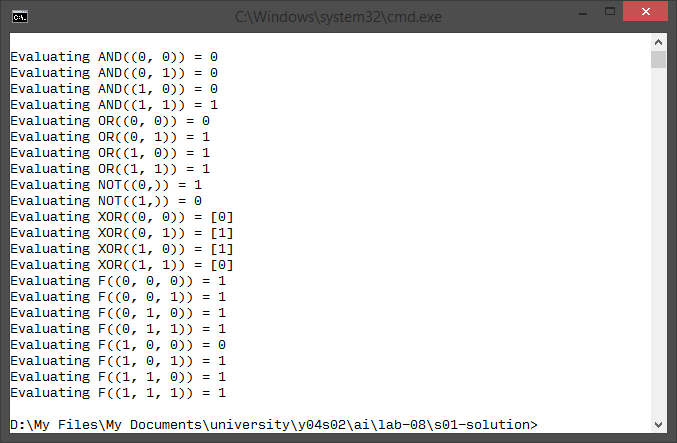
\includegraphics[width = 9\gridunitwidth]{./assets/y04s02-ai-lab-08-s02-report-p01.png}
      \caption{Результат роботи розробленої програми}
      \label{fig:res}
    \end{figure}

    Як~видно, розроблена програма коректно працює і~обчислює правильні результати як~для~логічних функцій, так~і~для~довільної функції, заданої таблицею істинності.

  \section{Висновок}
    Виконуючи дану лабораторну роботу, ми~отримали початкові навички по~створенню штучних нейронних мереж, що~здатні виконувати прості логічні функції.

  \appendix
  \section{Лістинг розробленої програми}
    \inputpython{../s01-solution/neuron.py}{Файл~\textenglish{\filename{neuron.py}}: модель нейронної мережі}{lst:neural-net}

    \inputpython{../s01-solution/main.py}{Файл~\textenglish{\filename{main.py}}: основний модуль}{lst:main}

\end{document}
